\documentclass[10pt]{article}
\usepackage[margin=0.75in]{geometry}
\usepackage{amsmath,amssymb}
\usepackage{graphicx}
\usepackage{booktabs}
\usepackage{float}
\usepackage[hidelinks]{hyperref}

\title{\vspace{-1.5em}EllipseNet: YOLO-Style Oriented Ellipse Detection}
\author{Hailemariam \quad NetID: hbm9834\\Applied Machine Learning Final Project}
\date{Spring 2026}

\begin{document}
\maketitle
\vspace{-1.5em}

\section{Project Requirements Covered}
The project modifies a YOLO-style detector to predict oriented ellipses instead of axis-aligned boxes. The implemented requirements are:
\begin{itemize}
    \item dataset customization: Pascal VOC boxes are converted to ellipse annotations;
    \item augmentation: training images are randomly rotated and ellipse centers/angles are updated;
    \item architecture change: the output head predicts ellipse parameters and class scores;
    \item IoU calculation: ellipse overlap is estimated and used for NMS/evaluation;
    \item loss integration: localization, objectness, classification, and angle losses are combined;
    \item hyperparameter search: learning rate, thresholds, and selected loss weights were tested;
    \item metrics and visualizations: mAP, precision, recall, loss curves, sample predictions, missed predictions, and false positives.
\end{itemize}

\section{Dataset and Target Representation}
For each VOC object with bounding box $(x_{\min},y_{\min},x_{\max},y_{\max})$, I define an inscribed ellipse
\[
c_x=\frac{x_{\min}+x_{\max}}{2W},\qquad
c_y=\frac{y_{\min}+y_{\max}}{2H},
\]
\[
a=\frac{x_{\max}-x_{\min}}{2W},\qquad
b=\frac{y_{\max}-y_{\min}}{2H},\qquad
\theta=0.
\]
During training, each image may be rotated by a random angle $\alpha$. The center is rotated around $(0.5,0.5)$ and the angle target becomes
\[
\theta'=(\theta+\alpha)\bmod \pi.
\]
Validation images are not randomly rotated, so validation measures performance on the original VOC distribution.

\begin{figure}[H]
\centering
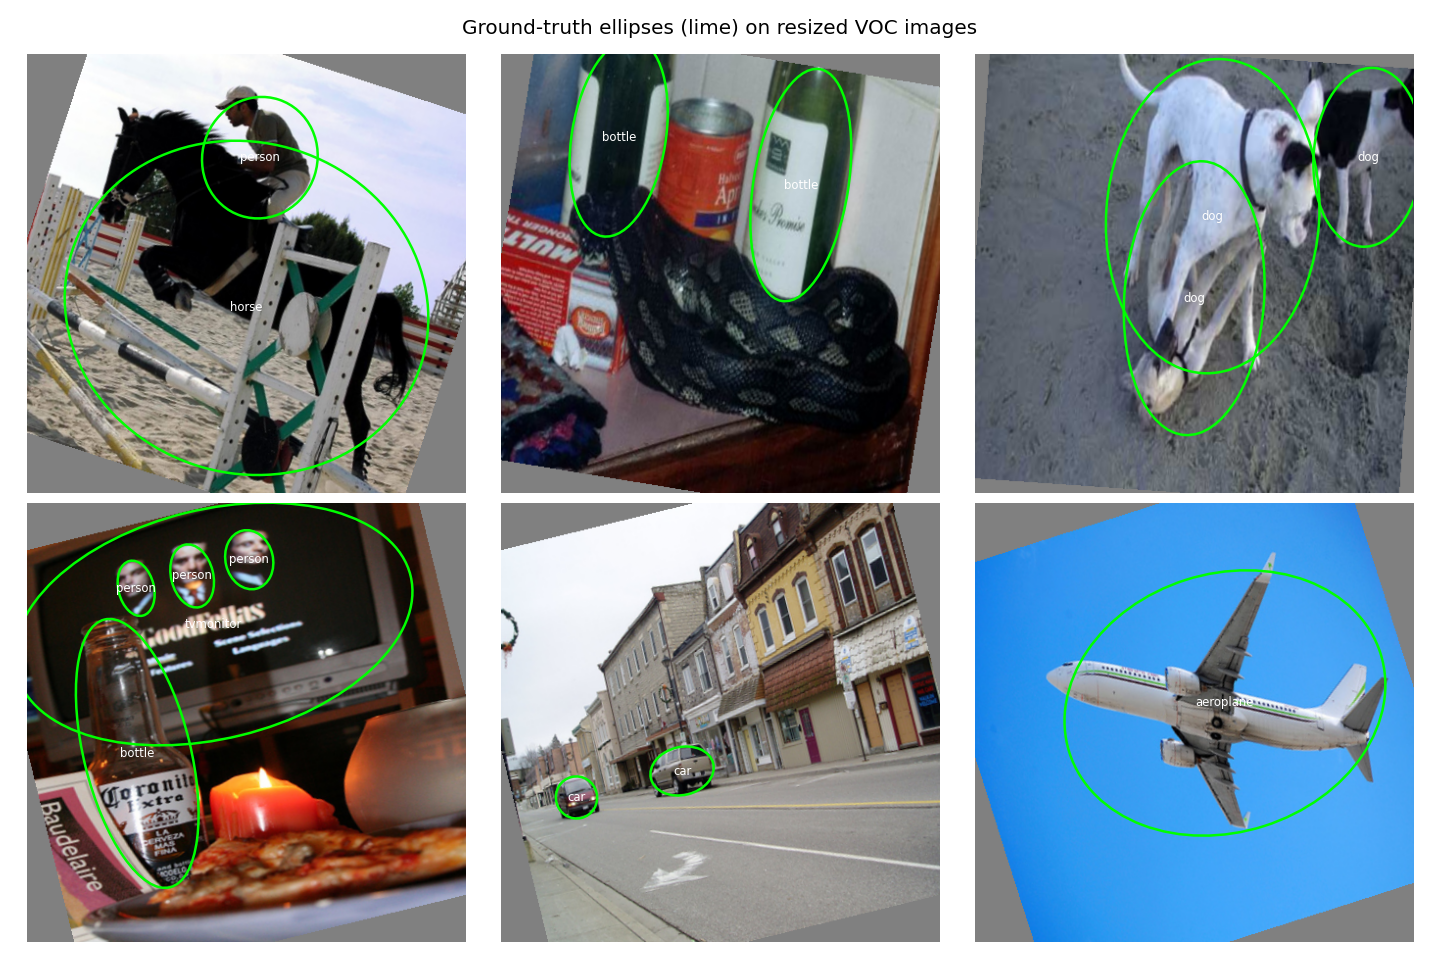
\includegraphics[width=0.47\linewidth]{figures/gt_ellipses.png}
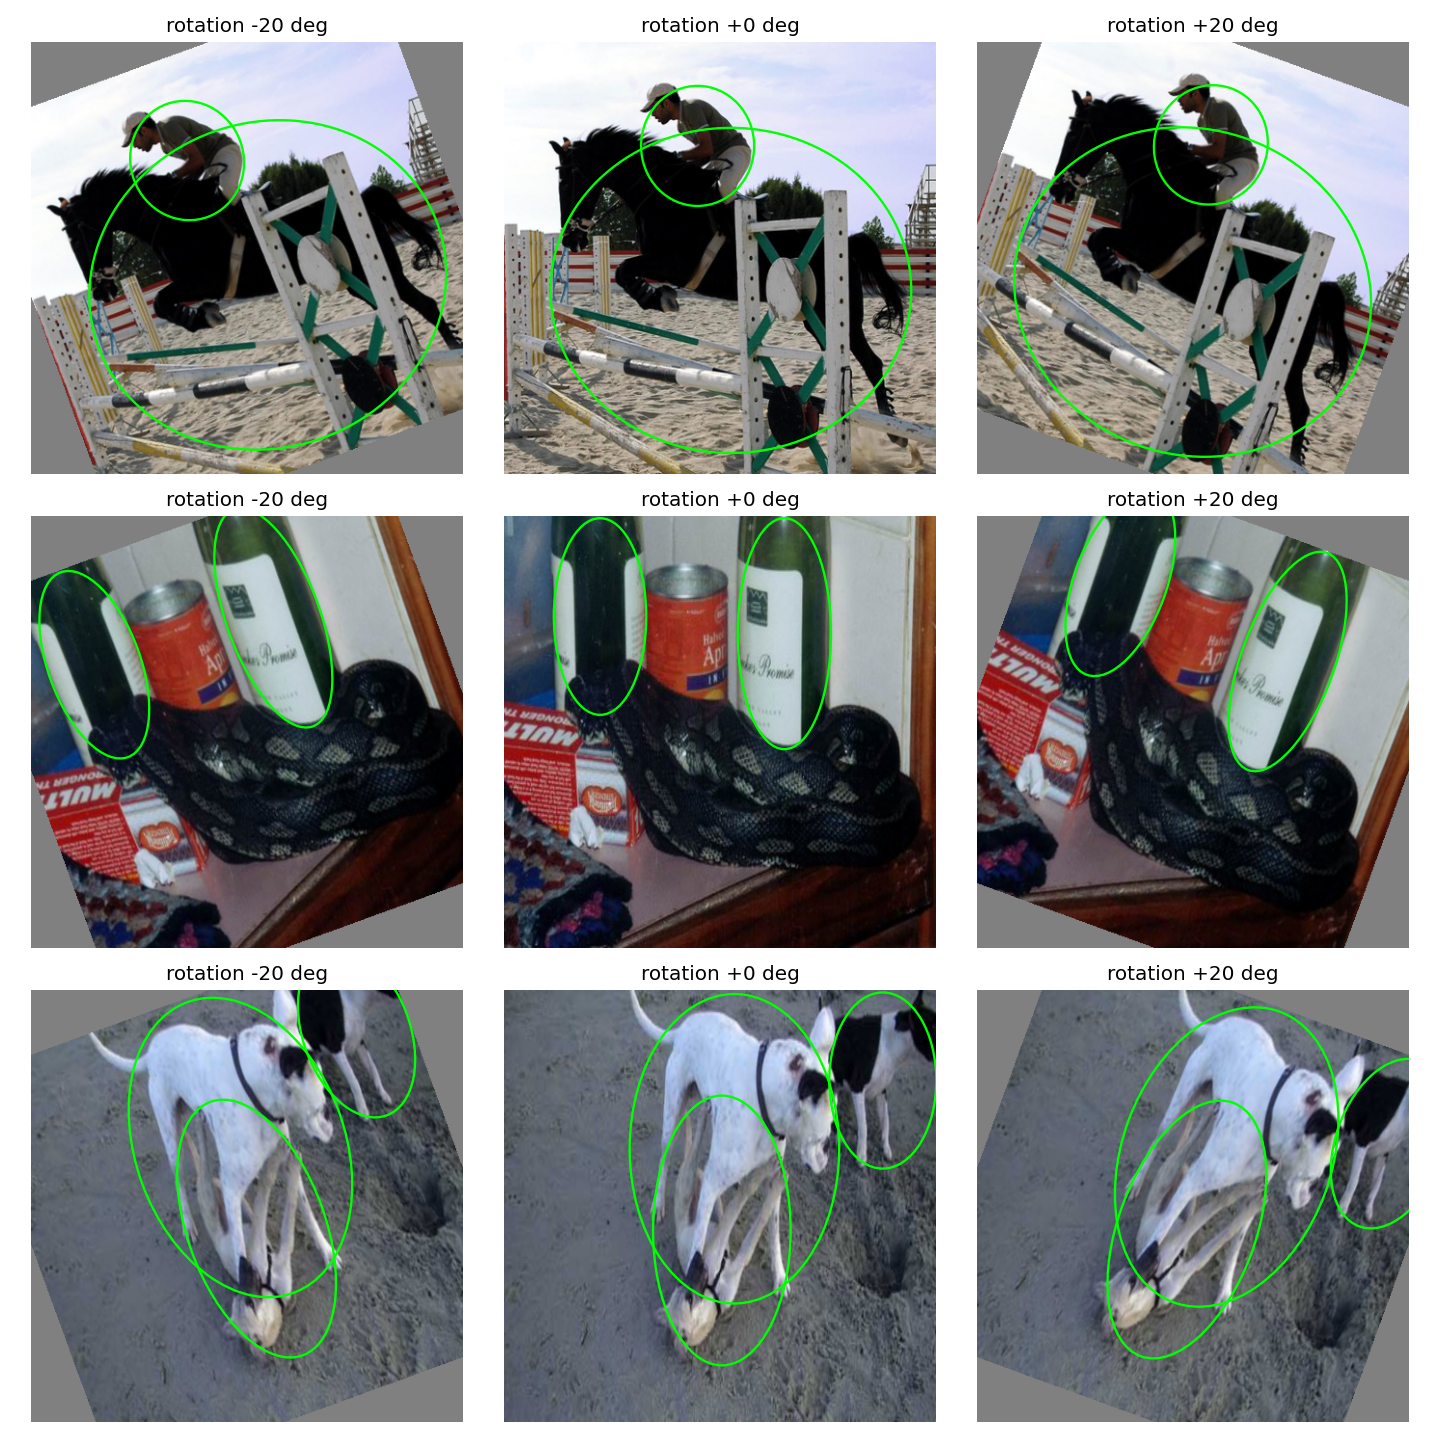
\includegraphics[width=0.47\linewidth]{figures/rotation_preview.png}
\caption{Ground-truth ellipse overlays and rotation augmentation checks.}
\end{figure}

\section{Model Architecture}
The final NumPy model uses input size $224\times224$, grid size $S=7$, $B=2$ ellipse predictors per cell, and $C=20$ VOC classes. The output tensor is
\[
7\times7\times2\times(6+20).
\]
For each cell-anchor pair, the model predicts
\[
(\hat{o},\hat{t}_x,\hat{t}_y,\hat{t}_a,\hat{t}_b,\hat{t}_{\theta},\hat{\mathbf{p}}_{cls}).
\]
The decoded ellipse is
\[
\hat{c}_x=\frac{\sigma(\hat{t}_x)+i}{S},\qquad
\hat{c}_y=\frac{\sigma(\hat{t}_y)+j}{S},
\]
\[
\hat{a}=A_a\exp(\hat{t}_a),\qquad
\hat{b}=A_b\exp(\hat{t}_b),\qquad
\hat{\theta}=\pi\sigma(\hat{t}_{\theta}),
\]
where $(A_a,A_b)$ is the assigned ellipse anchor. The final detection score is
\[
\text{score}=\sigma(\hat{o})\max_k \text{softmax}(\hat{\mathbf{p}}_{cls})_k.
\]

The implemented backbone is a small NumPy CNN:
\[
224\rightarrow112\rightarrow56\rightarrow28\rightarrow14\rightarrow7.
\]
It uses $3\times3$ convolutions, $1\times1$ bottleneck convolutions, max pooling, a fully connected hidden layer, and a final dense detection head. The final model has 2,992,188 scalar parameters.

\section{Loss Function and IoU}
Each ground-truth ellipse is assigned to the grid cell containing its center. The responsible anchor is selected by shape overlap between $(a,b)$ and the anchor axes. The total loss is
\[
\mathcal{L}=
\lambda_{loc}\mathcal{L}_{loc}
+\lambda_{obj}\mathcal{L}_{obj}
+\lambda_{noobj}\mathcal{L}_{noobj}
+\lambda_{cls}\mathcal{L}_{cls}
+\lambda_{\theta}\mathcal{L}_{\theta}.
\]
The localization loss combines center MSE, log-axis MSE, and a YOLO-style square-root axis term:
\[
\mathcal{L}_{loc}
=\|\sigma(\hat{t}_{xy})-t_{xy}\|_2^2
+\|\hat{t}_{ab}-t_{ab}\|_2^2
+\|\sqrt{\hat{a},\hat{b}}-\sqrt{a,b}\|_2^2.
\]
Objectness uses binary cross entropy, classification uses softmax cross entropy, and angle uses a $\pi$-periodic error:
\[
\mathcal{L}_{\theta}=\min(|\hat{\theta}-\theta|,\pi-|\hat{\theta}-\theta|).
\]
For evaluation and NMS, ellipse IoU is estimated by Monte Carlo sampling:
\[
\text{IoU}(E_1,E_2)\approx
\frac{\sum_{m=1}^{M}\mathbf{1}[p_m\in E_1\cap E_2]}
{\sum_{m=1}^{M}\mathbf{1}[p_m\in E_1\cup E_2]}.
\]

\section{Experiments and Results}
\subsection{Full From-Scratch Training}
The full run used all 5,717 VOC train samples and 5,823 validation samples. The best validation checkpoint occurred at epoch 9.

\begin{table}[H]
\centering
\begin{tabular}{lccc}
\toprule
Run & Train Loss & Val Loss & Note\\
\midrule
Epoch 1 & 5.7543 & 5.2136 & initial\\
Best checkpoint & 3.5350 & 4.6092 & epoch 9\\
Epoch 30 & 1.4056 & 5.2631 & overfitting\\
\bottomrule
\end{tabular}
\caption{Full from-scratch training loss.}
\end{table}

\begin{table}[H]
\centering
\begin{tabular}{lccc}
\toprule
Split & mAP & Precision & Recall\\
\midrule
Train & 0.0859 & 0.1462 & 0.1333\\
Validation & 0.0560 & 0.0960 & 0.0996\\
\bottomrule
\end{tabular}
\caption{Ellipse-IoU evaluation on the best checkpoint.}
\end{table}

\begin{figure}[H]
\centering
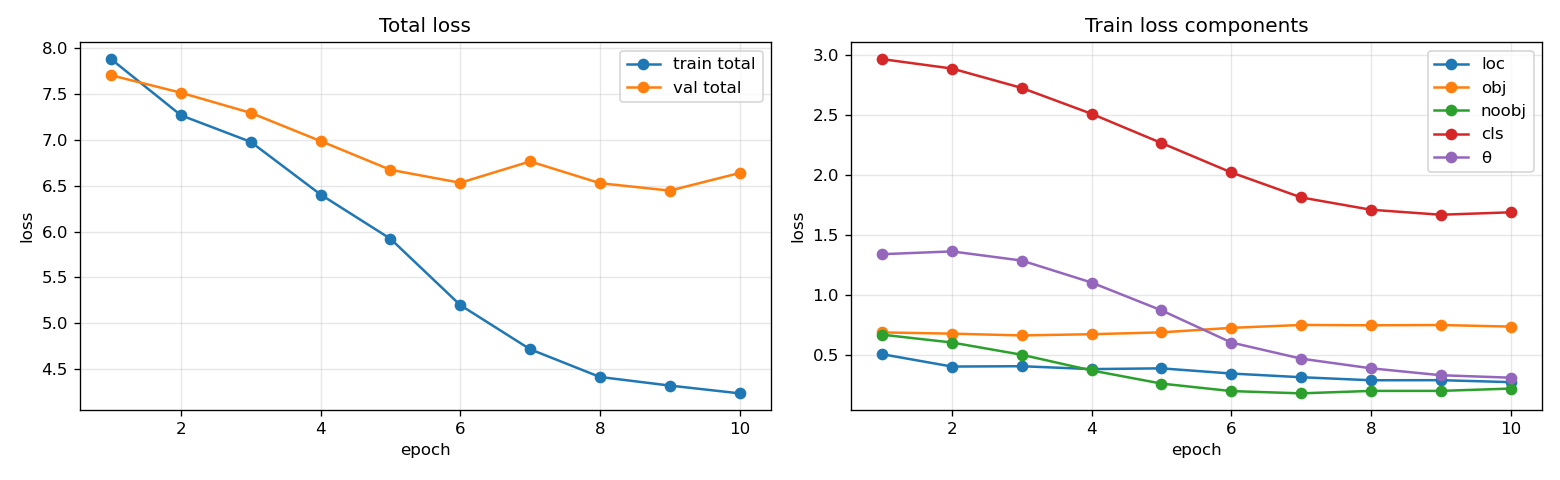
\includegraphics[width=0.55\linewidth]{figures/loss_curves.png}
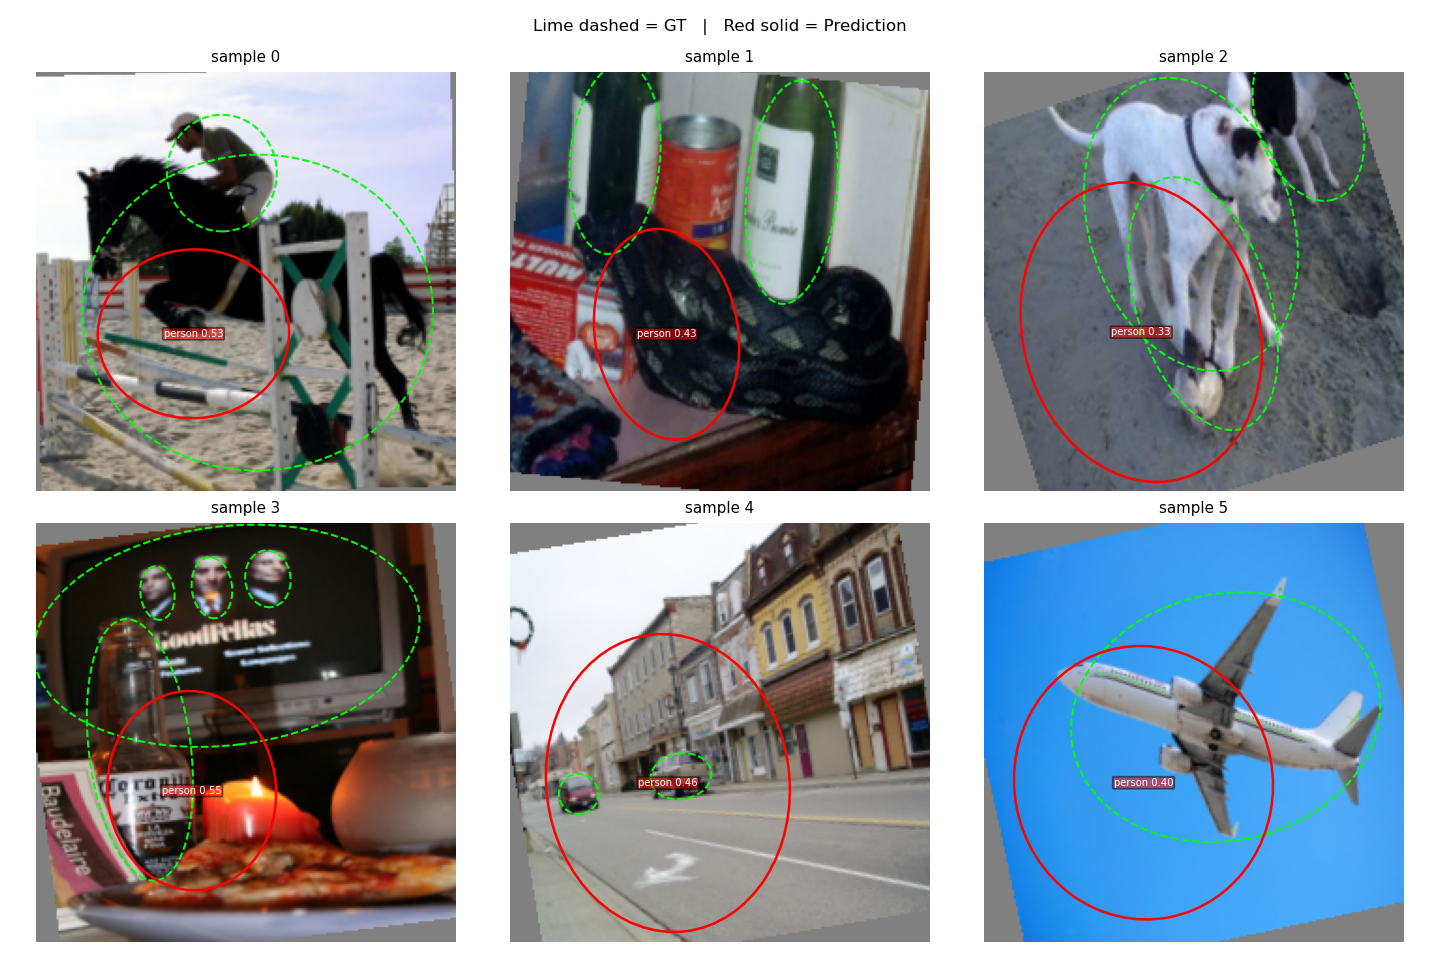
\includegraphics[width=0.40\linewidth]{figures/train_preds.png}
\caption{Full training loss curve and sample predictions.}
\end{figure}

\subsection{Hyperparameter Tests}
Learning-rate and confidence-threshold experiments were run on a staged dataset. The best staged validation loss among the tested learning rates was obtained with $5\times10^{-4}$.

\begin{table}[H]
\centering
\begin{tabular}{lccc}
\toprule
Learning Rate & Best Val Loss & Best Conf. & Best mAP\\
\midrule
$1\times10^{-3}$ & 6.3755 & 0.3 & 0.0001\\
$5\times10^{-4}$ & 6.3055 & 0.3 & 0.0002\\
$1\times10^{-4}$ & 6.8470 & 0.3 & 0.0000\\
\bottomrule
\end{tabular}
\caption{Staged hyperparameter search.}
\end{table}

\begin{figure}[H]
\centering
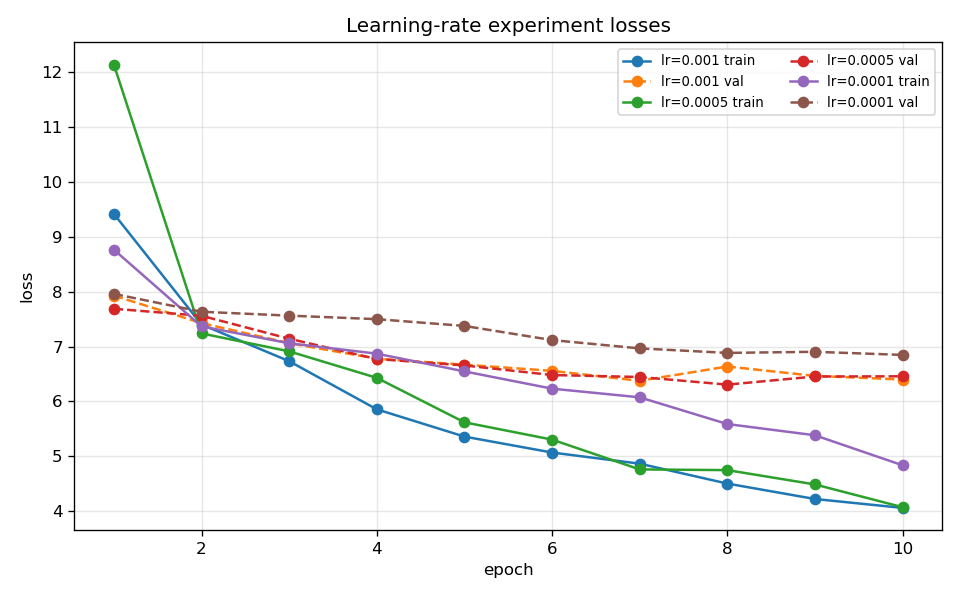
\includegraphics[width=0.48\linewidth]{figures/clean2_lr_experiment_losses.png}
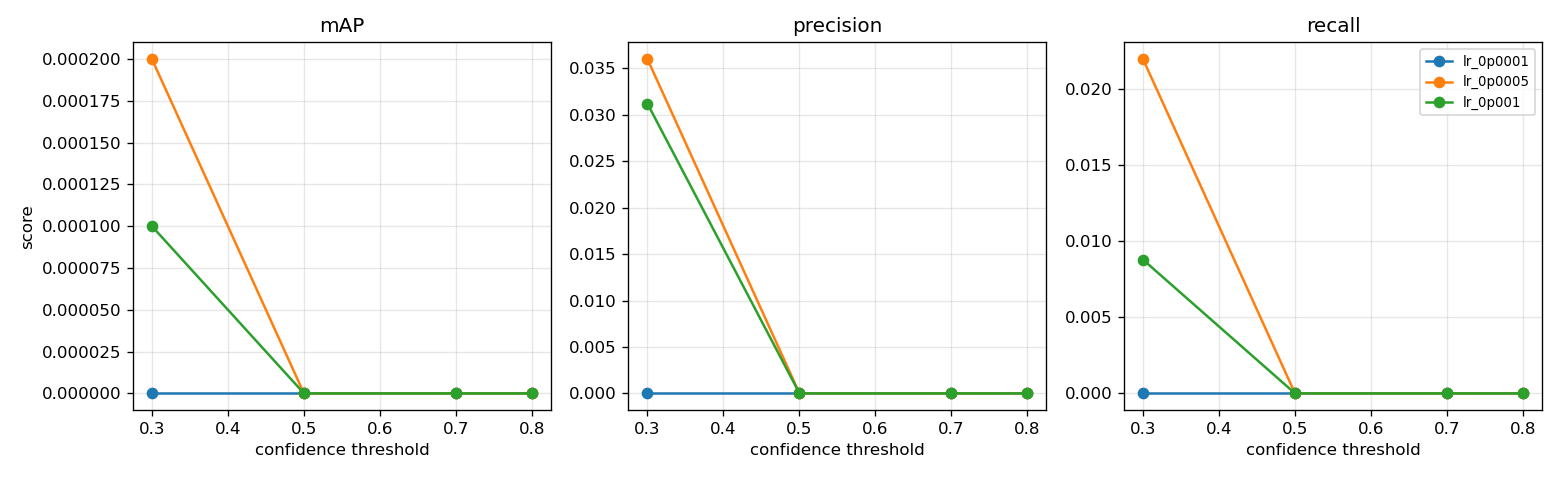
\includegraphics[width=0.48\linewidth]{figures/clean2_threshold_summary.png}
\caption{Learning-rate test curves and threshold sweep summary.}
\end{figure}

\subsection{Overfitting Check}
A 20-image deterministic overfitting run was used to verify that the model and training pipeline can memorize a small dataset. The loss dropped strongly, confirming that gradient flow, target assignment, decoding, and visualization are working.

\begin{table}[H]
\centering
\begin{tabular}{lcc}
\toprule
Epoch & Train Loss & Val Loss\\
\midrule
1 & 19.8149 & 9.6162\\
20 & 1.7805 & 1.4900\\
\bottomrule
\end{tabular}
\caption{Twenty-image overfitting result.}
\end{table}

\begin{figure}[H]
\centering
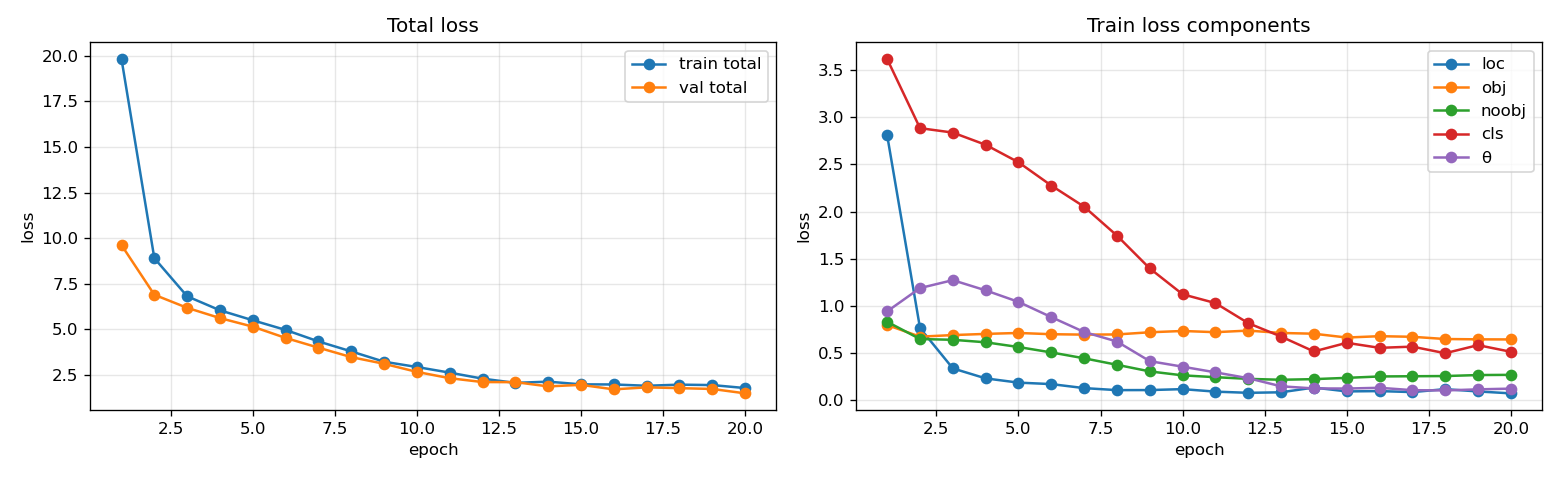
\includegraphics[width=0.48\linewidth]{figures/final_overfitting_loss.png}
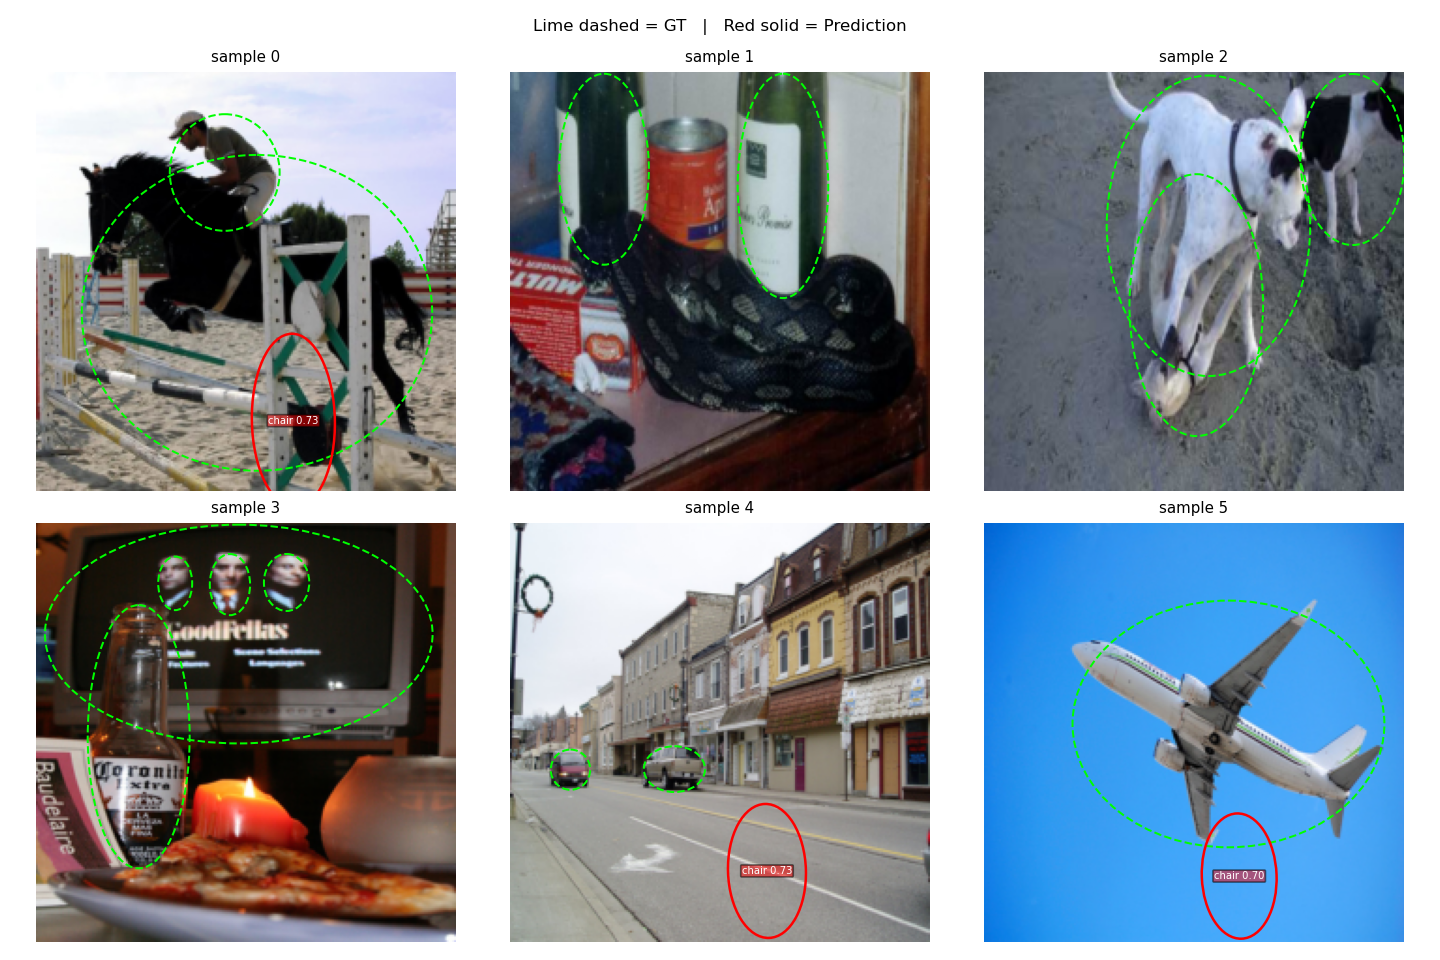
\includegraphics[width=0.48\linewidth]{figures/final_overfitting_predictions.png}
\caption{Overfitting loss curve and predictions after the overfit check.}
\end{figure}

\subsection{Pretrained Backbone Experiment}
I also implemented an advanced version with an ImageNet-pretrained ResNet-18 backbone. The original classifier is removed, a new ellipse detection head is attached, the backbone is frozen for the first epochs, and then all layers are fine-tuned. The current pretrained notebook supports $448\times448$ input and uses adaptive pooling to preserve a $7\times7$ output grid.

A staged pretrained run improved validation loss to 3.6745. Its threshold sweep showed higher recall than the NumPy-from-scratch model:
\begin{table}[H]
\centering
\begin{tabular}{lccc}
\toprule
Confidence & mAP & Precision & Recall\\
\midrule
0.30 & 0.0617 & 0.0528 & 0.3297\\
0.50 & 0.0538 & 0.1036 & 0.2817\\
0.70 & 0.0409 & 0.1738 & 0.2227\\
\bottomrule
\end{tabular}
\caption{Pretrained ResNet-18 backbone validation threshold sweep.}
\end{table}

\begin{figure}[H]
\centering
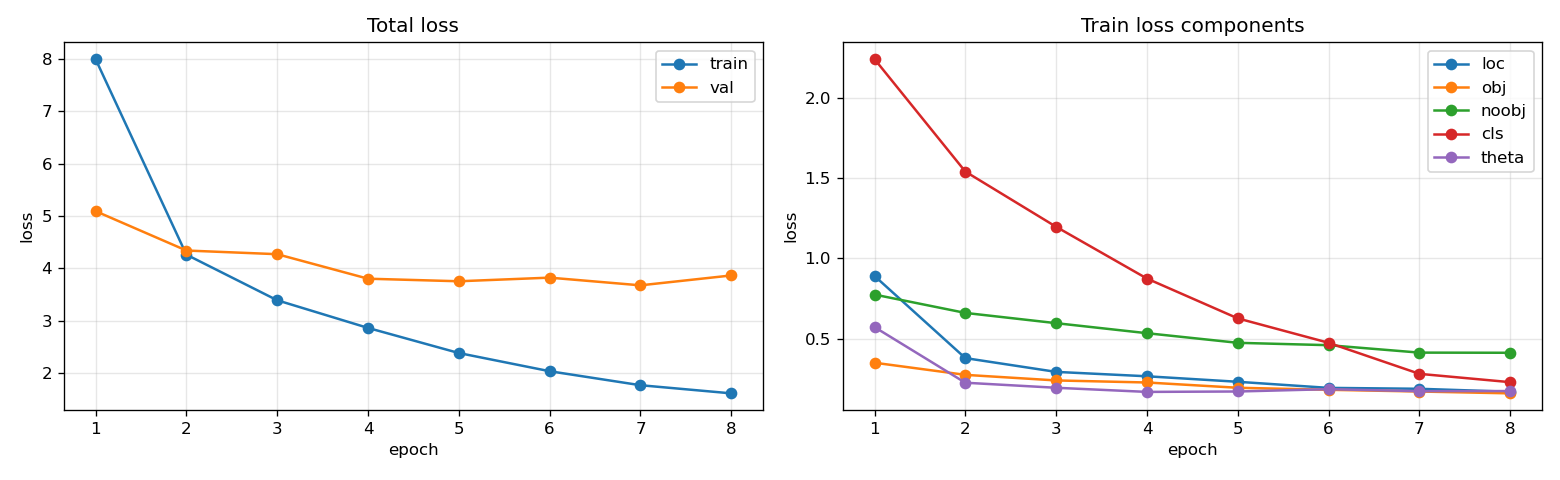
\includegraphics[width=0.48\linewidth]{figures/pretrained_loss_curves.png}
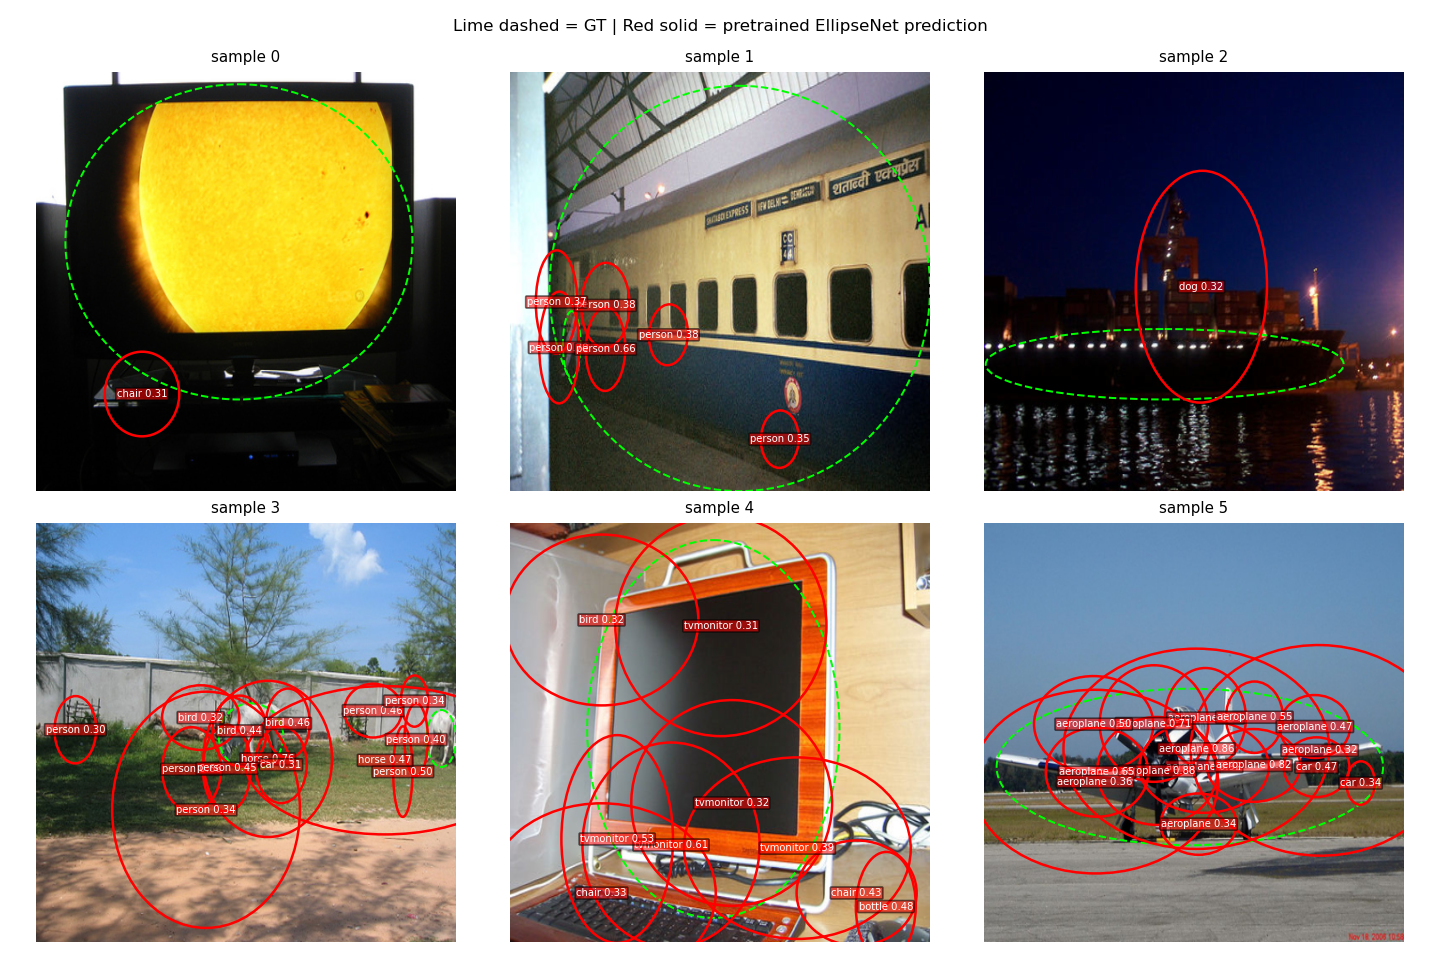
\includegraphics[width=0.48\linewidth]{figures/pretrained_predictions.png}
\caption{Pretrained backbone training curve and predictions.}
\end{figure}

\section{Conclusion}
The final detector satisfies the required project components: VOC annotation customization, ellipse output modification, IoU/NMS, integrated loss, hyperparameter search, mAP evaluation, and prediction visualizations. The from-scratch NumPy model trains correctly and can overfit a small set, but full VOC performance is limited by training from scratch, small model capacity, confidence calibration, and noisy ellipse targets derived from boxes. The pretrained ResNet-18 version improves feature quality and recall, showing that pretrained backbones are a practical next step for better detection performance.

\end{document}
